\appendix

\begin{frame}[noframenumbering, plain]{}
    Backup slides
\end{frame}

% XXX write those
\begin{frame}{MR signal derivation}
    \only<1>{
        Bloch equations:
        \begin{equation*}
            \begin{split}
                \diff{\Mb_{tr}}{t} &= - \frac{ \tikzmarknode{mtr}{\Mb_{tr}} }{T_2} \\
            \diff{\Mb_l}{t} &= \frac{ \tikzmarknode{mo}{\Mb_0}  - \tikzmarknode{ml}{\Mb_l} }{T_1}
            \end{split}
        \end{equation*}

        \vspace{4em}
        \begin{tikzpicture}[overlay,remember picture,>=stealth,nodes={align=left,inner ysep=1pt},<-]
            % For "mtr"
            \path (mtr.north) ++ (0,2em) node[anchor=south west,color=black!87] (exp_mtr){
                \textbf{Transverse component of $\Mb$}};
            \draw [color=black!87](mtr.north) |- ([xshift=-0.3ex,color=black]exp_mtr.south east);
            % For "mo"
            \path (mo.south) ++ (0, -4em) node[anchor=south east,color=black!87] (exp_mo){
                \textbf{Equilibrium state}};
            \draw [color=black!87](mo.south) |- ([xshift=-0.3ex,color=black]exp_mo.south west);
            % For "ml"
            \path (ml.south) ++ (0,-4em) node[anchor=south west,color=black!87] (exp_ml){
                \textbf{Longitudinal component of $\Mb$}};
            \draw [color=black!87](ml.south) |- ([xshift=-0.3ex,color=black]exp_ml.south east);
        \end{tikzpicture}
    }
    \only<2>{
        Solution:
        \begin{equation*}
            \begin{split}
                \Mb_{tr}(t, \rb) &= \tikzmarknode{mtro}{\Mb_{tr}(0, \rb)} e^{-\frac{t}{T_2}}\\
                \Mb_l(t, \rb) &= \Mb_l(0, \rb) e^{-\frac{t}{T_1}} + \Mb_0 (1 - e^{-\frac{t}{T_1}})
            \end{split}
        \end{equation*}
        \vspace{4em}
        \begin{tikzpicture}[overlay,remember picture,>=stealth,nodes={align=left,inner ysep=1pt},<-]
            % For "mtro"
            \path (mtro.north) ++ (0, 2em) node[anchor=south west,color=black!87] (exp_mtro){
                $|\Mb_{tr}(0, \rb)| = \frac14 \rho(\rb) \frac{\gamma^2 \hbar^2}{kT}B_0$};
            \draw [color=black!87](mtro.north) |- ([xshift=-0.3ex,color=black]exp_mtro.south east);
        \end{tikzpicture}
    }
    \only<3>{
        EF force in antenna:
        \begin{equation*}
            S(t) = - \diff{}{t} \int_{V_s} \Bb_1 \cdot \Mb(t, \rb) \dif \rb
        \end{equation*}
    }

\end{frame}

\begin{frame}{Fourier Transform and MRI}
    \begin{multicols}{2}
        MR signal:
        \begin{equation*}
            \vspace{\baselineskip}
            S_{tr}(t) \propto \omega_0  \int_{V_s} B_{tr} M_{tr}(t, \rb) e^{-\imath \gamma \rb \cdot \int_0^t \Gb(\tau)  \dif \tau} \dif \rb
        \end{equation*}
        \newpage
        Fourier Transform of a signal:
        \begin{equation*}
            \hat{f}(\omega) = \int_{-\infty}^{\infty} f(x) e^{-2\pi \imath \omega x} dx
        \end{equation*}
    \end{multicols}
\end{frame}

\begin{frame}{More details on GRAPPA}

\end{frame}

\begin{frame}{Sparsity}

\end{frame}

\begin{frame}{Basis Pursuit}

\end{frame}

\begin{frame}{Sensitivity Maps}

\end{frame}

\begin{frame}{Noise model for MRI}

\end{frame}

\begin{frame}{Proximity operator}
    Definition:
    \begin{equation*}
        \operatorname{prox}_{\mathcal{R}}(\xb) = \argmin_{\zb \in \mathcal{H}} \mathcal{R}(\zb) + \frac12\|\zb - \xb\|_2^2
    \end{equation*}
    2 intuitions:
    \begin{itemize}
        \item Prox. of indicator of $\mathcal{C}$, a convex set, is the projection onto $\mathcal{C}$.
        \item Prox. of a smooth function is its gradient step.
    \end{itemize}
\end{frame}

\begin{frame}{Convolutions}

\end{frame}

\begin{frame}{CNN}
    Convolutional Neural Network~(CNN): chain of Convolution + Nonlinearity.
\end{frame}

\begin{frame}{U-net}
    \begin{figure}
        \centering
        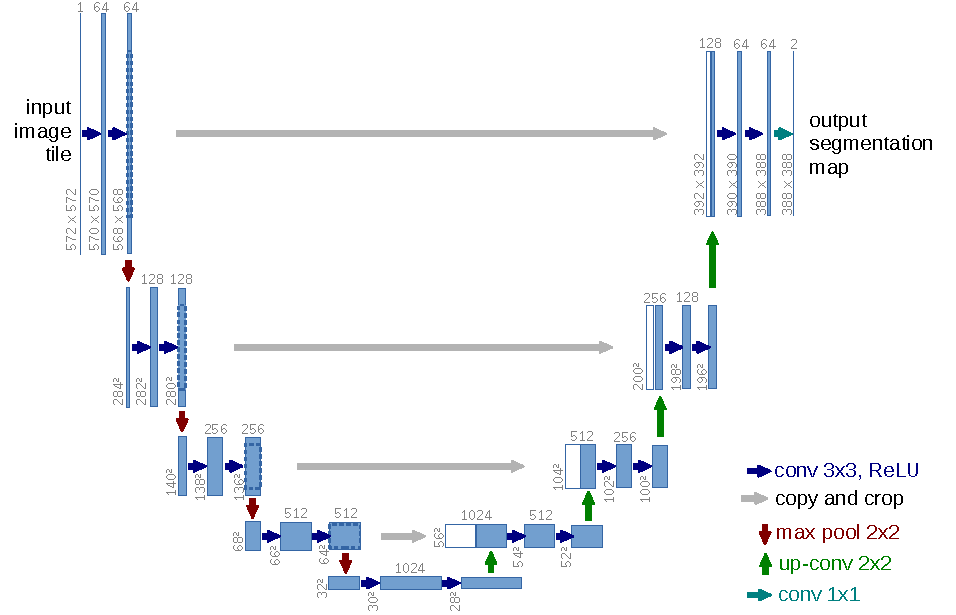
\includegraphics[height=0.6\textheight]{Figures/add_slides/unet_hires.pdf}
        \caption{Illustration from the original paper.\footfullcite{ronneberger2015u}}
    \end{figure}
\end{frame}

\begin{frame}{MWCNN}
    \begin{figure}
        \centering
        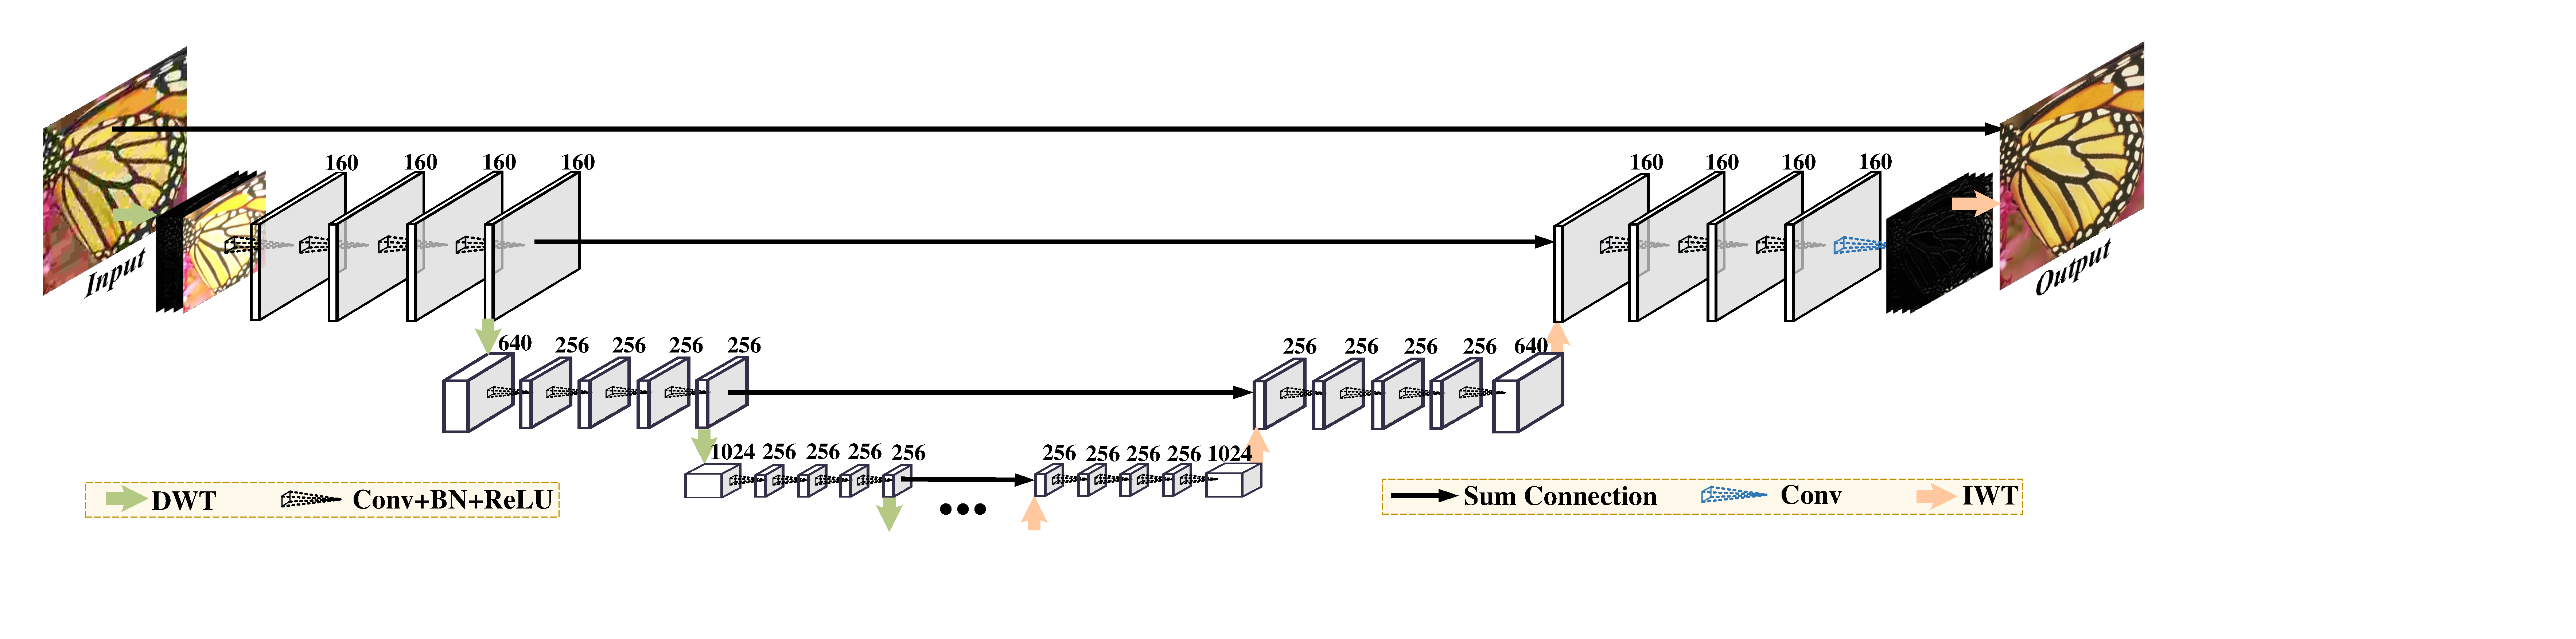
\includegraphics[width=\textwidth]{Figures/add_slides/mwcnn.pdf}
        \caption{Illustration from the original paper.\footfullcite{Liu2018}}
    \end{figure}
\end{frame}

\begin{frame}{fastMRI dataset}
    \href{https://fastmri.org/}{fastmri.org}
    \begin{multicols}{2}
        \textbf{Knee}
        \begin{itemize}
            \item 973 train volumes, 199 validation volumes
            \item 2 contrasts: PD and PDFS
            \item 15 coils, 1.5T/3T, 320x320, 0.5mmx0.5mm, Cartesian 2D TSE
        \end{itemize}
        \newpage
        \textbf{Brain}
        \begin{itemize}
            \item 4469 train volumes, 1378 validation volumes
            \item 4 contrasts: T1, T1 post injection, T2, FLAIR
            \item different locations, different coil architecture
            \item 1.5T/3T, 320x320 (with exceptions), 0.5mmx0.5mm, Cartesian 2D TSE
        \end{itemize}
    \end{multicols}
\end{frame}

\begin{frame}{2020 fastMRI challenge}
    \begin{itemize}
        \item 2nd edition
        \item 8 teams
        \item Brain data
        \item 3 tracks: 4X, 8X, transfer
    \end{itemize}
\end{frame}

\begin{frame}{What did the winners do that I did not}
    \begin{itemize}
        \item Unclear feature multi-domain learning
        \item 3D Post-processing (main network is 2D)
        \item Distributed training (4 GPUs)
    \end{itemize}
\end{frame}

\begin{frame}{autoMAP}
    \begin{figure}
        \centering
        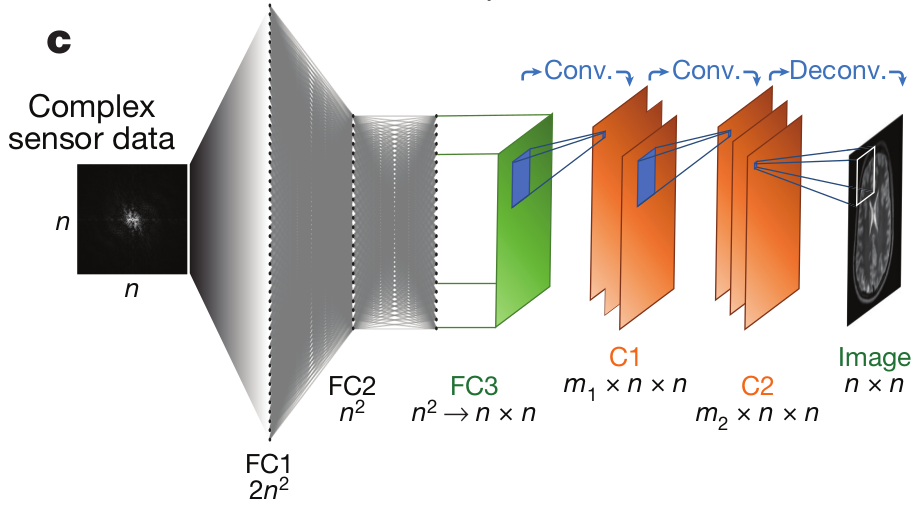
\includegraphics[width=0.67\textwidth]{Figures/add_slides/automap.png}
        \caption{Illustration from the original paper.\footfullcite{Zhu2018}}
    \end{figure}
\end{frame}

\begin{frame}{XPDNet - ct'ed}
    \begin{center}
        \scalebox{0.85}{
        \begin{algorithm}[H]
            \SetAlgoLined
            \KwData{$\ybb$ the k-space data, $\Omega$ the Cartesian trajectory, $\Sbb$ the coarse estimates of the sensitivity maps}
            \KwResult{$\xb$, the reconstructed magnitude MR image}
             $\Sbb = g_{\theta_r}(\Sbb)$ ; \tcp{Sensitivity maps refinement}
             Update ${\cal A}$ and ${\cal A}^H$\;
             $\xb =  {\cal A}^H \ybb$\;

             $\xb_b = [\xb, \xb, \xb, \xb, \xb]$; \tcp{Buffer creation, in practice concatenation along the channel dimension}
             \For{$i \leftarrow 1$ \KwTo $N_C$}{
               $\ybb_{res} = {\cal A}\, \xb_b[0] - \ybb $; \tcp{Data consistency}
              $\xb_{dc} = {\cal A}^H \ybb_{res}$; \tcp{Density compensation}
              $\xb_b = \xb_b + f_{\theta_i}([\xb_b, \xb_{dc}]))$; \tcp{Proximity operator learning and nonlinear acceleration scheme}
             }
             $\xb = |\xb_b[0]|$ \tcp{Magnitude computation}
             \caption{\emph{XPDNet}.}
        \end{algorithm}
    }
    \end{center}
\end{frame}

\begin{frame}{PDNet \& Recurent Inference Machines~(RIMs)}
    Bayesian Inverse Problem formulation:
    \begin{equation*}
        \argmax_x p(x|y) \propto p(y|x) p(x)
    \end{equation*}
    Updates:
    \begin{equation*}
        x_{n+1} = x_n + \epsilon_n \nabla_x (\log p(y|x) + \log p(x))(x_n)
    \end{equation*}
    RIMs generalize to:\footfullcite{Putzky2017RecurrentProblems}
    \begin{equation*}
        x_{n+1} = x_n + g(\nabla_x(\log p(y|x))(x_n), x_n)
    \end{equation*}
\end{frame}

\begin{frame}{NC-PDNet - ct'ed}
    \begin{center}
        \scalebox{0.85}{
        \begin{algorithm}[H]
            \SetAlgoLined
            \KwData{$\ybb$ the k-space data, $\Omega$ the non-Cartesian trajectories, $\db$ the pre-computed DCp weights, $\Sbb$ the coarse estimates of the sensitivity maps}
            \KwResult{$\xb$, the reconstructed magnitude MR image}
             $\Sbb = g_{\theta_r}(\Sbb)$ ; \tcp{Sensitivity maps refinement}
             Update ${\cal A}$ and ${\cal A}^H$\;
             $\xb =  {\cal A}^H \ybb$\;

             $\xb_b = [\xb, \xb, \xb, \xb, \xb]$; \tcp{Buffer creation, in practice concatenation along the channel dimension}
             \For{$i \leftarrow 1$ \KwTo $N_C$}{
               $\ybb_{res} = {\cal A}\, \xb_b[0] - \ybb $; \tcp{Data consistency}
              $\xb_{dc} = {\cal A}^H \db\, \ybb_{res}$; \tcp{Density compensation}
              $\xb_b = \xb_b + f_{\theta_i}([\xb_b, \xb_{dc}]))$; \tcp{Proximity operator learning and nonlinear acceleration scheme}
             }
             $\xb = |\xb_b[0]|$ \tcp{Magnitude computation}
             \caption{\emph{NC-PDNet}: Density compensated Primal Dual unrolled neural network over $N_C$ iterations.}
             \label{alg:NC-PDNet}
        \end{algorithm}
    }
    \end{center}
\end{frame}

\begin{frame}{Density Compensation}
    \begin{equation*}
            \db_{n+1} = \frac{\db_n}{{\cal F}_{\Omega} {\cal F}^H_{\Omega} \db_n}
    \end{equation*}
\end{frame}

\begin{frame}{Image quality metrics}
    \begin{multicols}{2}
        \textbf{Peak Signal to Noise Ratio~(PSNR)}:
        \begin{equation*}
            \operatorname{PSNR}(\xb, \hat{\xb}) = 10 \log_{10}\left( \frac{\max_i{\xb_i}}{\frac1n \|\xb - \hat{\xb}\|^2_2}\right)
        \end{equation*}
        \newpage
        \textbf{Structural Similarity Index~(SSIM)}:
        \begin{equation*}
            \operatorname{SSIM}(\xb, \hat{\xb}) = [l(\xb, \hat{\xb})]^\alpha . [c(\xb, \hat{\xb})]^\beta . [s(\xb, \hat{\xb})]^\gamma
        \end{equation*}
        \begin{itemize}
            \item $l$: luminance
            \item $c$: contrast
            \item $s$: structure
        \end{itemize}
    \end{multicols}
    Problem: not a good correlation with the actual visual quality.
\end{frame}

\begin{frame}{quasi-Newton methods - 1}
    Idea: replace the costly Jacobian inverse with a qN matrix $\Bb^{-1}$.\\
    \begin{equation*}
        f(x^\star) = 0
    \end{equation*}
    \begin{multicols}{2}

            \begin{center}
                \textbf{Newton Methods}
                \begin{equation*}
                    x_{n+1} = x_n -\frac{\partial f}{\partial x}(x_n)^{-1}f(x_n)
                \end{equation*}
            \end{center}
            \newpage
            \begin{center}
                \textbf{Quasi-Newton Methods}
                \begin{equation*}
                    x_{n+1} = x_n -\Bb_n^{-1}f(x_n)
                \end{equation*}
            \end{center}
            Update $\Bb_n$ and its inverse with the Sherma-Morrison formula.
    \end{multicols}
\end{frame}

\begin{frame}{quasi-Newton methods - 2}
    Secant conditions: set of conditions $\Bb$ must verify.\\
    Typically: $\Bb_n(x_n - x_{n-1}) = f(x_n) - f(x_{n-1})$.\\
    Multiple solutions $\Rightarrow$ regularization with $\Bb_n = \argmin_{\Bb: \Bb \Delta x_n = \Delta f_n} \|\Bb - \Bb_{n-1}\|$
\end{frame}

\begin{frame}{OPA - 1}
    Outer Problem Awareness: modify the inner problem resolution depending on the outer problem.\\

    Additional updates of $\Bb$ with the OPA direction: $\eb_n = t_n \Bb_n^{-1} \frac{\partial g_{\theta}}{\partial \theta}\Bigr|_{\zb_n}$.
\end{frame}

\begin{frame}{OPA - 2}
    \begin{center}
        \scalebox{.5}{
    \begin{algorithm}[H]
        \SetAlgoRefName{LBFGS}
        \DontPrintSemicolon
        \caption{(Limited memory) BFGS method with OPA.}
        \label{alg:LBFGS}
        \KwIn{ initial guess $(\zb_0, \Bb_0^{-1})$, where $\Bb_0^{-1}$ is symmetric and positive definite, tolerance $\epsilon>0$, frequency of additional updates $M\in\mathbb{N}$, memory limit $L\in\mathbb{N}\cup\{\infty\}$, $(t_n)$ a null sequence of positive numbers with $\sum_n t_n<\infty$	}
        Let $F := \nabla_\zb g_{\theta}$\\
        \For{ $n=0,1,2,\ldots$ }
        {
            \lIf{$\norm{F(\zb_n)}\leq\epsilon$ }{let $\zb^\star:=\zb_n$ and let $\Bb:=\Bb_n$; STOP}
            Let $\hat \Bb_n^{-1}:=\Bb_n^{-1}$\\
            \If{$(n\operatorname{mod} M)=0$}{let $\eb_n:=t_n \Bb_n^{-1} \frac{\partial g_{\theta}}{\partial \theta}\Bigr|_{\zb_n}$,
                $\hat \yb_n:=F(\zb_n+\eb_n)-F(\zb_n)$ and $\hat \rb_n:=(\eb_n)^\top \hat \yb_n$\\
            \If{$\hat \rb_n>0$}{let $\hat \ab_n:=\eb_n - \Bb_n^{-1} \hat \yb_n$ and let
            \begin{equation*}
                \hat \Bb_n^{-1} := \Bb_n^{-1} + \frac{\hat \ab_n (\eb_n)^\top + \eb_n (\hat \ab_n)^\top}{\hat \rb_n} -
                \frac{(\hat \ab_n)^\top \hat \yb_n}{(\hat \rb_n)^2} \eb_n (\eb_n)^\top
            \end{equation*}
            }
        }
            Let $\Bb_n^{-1}:=\hat \Bb_n^{-1}$\\
            \lIf{$n\geq L$}{remove update $n-L$ from $\Bb_n^{-1}$}
            Let $p_n := -\Bb_n^{-1} F(\zb_n)$\\
            Obtain $\alpha_n$ via line-search and let $\sb_n := \alpha_n p_n$\\
            Let $\zb_{n+1}:=\zb_n+\sb_n$, $\yb_n:=F(\zb_{n+1})-F(\zb_n)$ and $\rb_n:=(\sb_n)^\top \yb_n$\\
            \uIf{$\rb_n>0$}{let $\ab_n:=\sb_n-\Bb_n^{-1} \yb_n$ and let
            \begin{equation*}
                \Bb_{n+1}^{-1} := \Bb_n^{-1} + \frac{\ab_n (\sb_n)^\top + \sb_n (\ab_n)^\top}{\rb_n} -
                \frac{(\ab_n)^\top \yb_n}{(\rb_n)^2} \sb_n (\sb_n)^\top
            \end{equation*}
            }
            \lElse{let $\Bb_{n+1}^{-1}:=\Bb_n^{-1}$}
            \lIf{$n\geq L$}{remove update $n-L$ from $\Bb_{n+1}^{-1}$}
        }
        \KwOut{$\zb^\star$, $\Bb$}
    \end{algorithm}
    }
    \end{center}
\end{frame}

\begin{frame}{Adjoint Broyden}
    For DEQs, vanilla OPA direction involves $\frac{\partial g_{\thetab}}{\partial \thetab}\Bigr|_{\zb_n}$ $\Rightarrow$ inefficient.\\

    Recall that the SHINE direction is: $\pb_\thetab =  \highlight{blue}{$\nabla_\zb \mathcal{L}(\zb^\star)$} B^{-1} \frac{\partial g_{\thetab}}{\partial \thetab}\Bigr|_{\zb^\star}$.\\
    Other direction, \highlight{blue}{$\nabla_\zb \mathcal{L}(\zb^\star)$}, in left-multiplication $\Rightarrow$ Adjoint Broyden for the secant condition to work.
\end{frame}

\begin{frame}{Jacobian-Free}
    \begin{equation*}
        \alt<2>{\Ib}{\Bb^{-1}} \approx J_{g_{\thetab}}(\zb^\star)^{-1}
    \end{equation*}
\end{frame}